% Created by tikzDevice version 0.12.6 on 2024-11-19 16:55:48
% !TEX encoding = UTF-8 Unicode
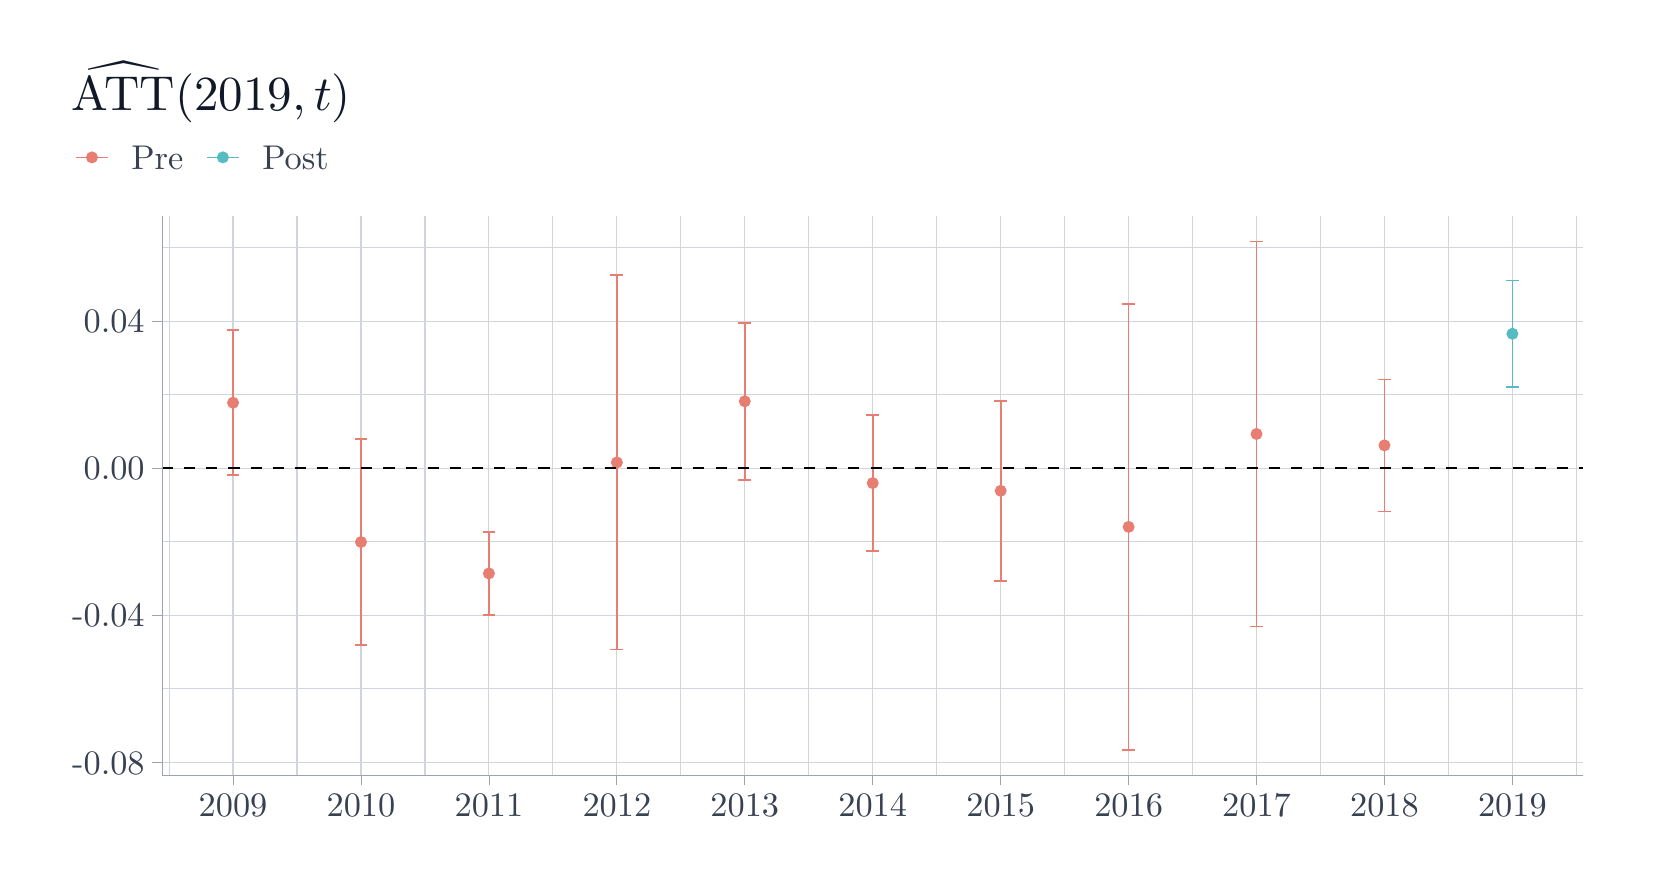
\begin{tikzpicture}[x=1pt,y=1pt]
\definecolor{fillColor}{RGB}{255,255,255}
\path[use as bounding box,fill=fillColor] (0,0) rectangle (578.16,303.53);
\begin{scope}
\path[clip] (  0.00,  0.00) rectangle (578.16,303.53);
\definecolor{drawColor}{RGB}{255,255,255}

\path[draw=drawColor,line width= 0.7pt,line join=round,line cap=round,fill=fillColor] (  0.00,  0.00) rectangle (578.16,303.53);
\end{scope}
\begin{scope}
\path[clip] ( 48.56, 33.29) rectangle (562.16,235.43);
\definecolor{drawColor}{RGB}{255,255,255}
\definecolor{fillColor}{RGB}{255,255,255}

\path[draw=drawColor,line width= 0.7pt,line join=round,line cap=round,fill=fillColor] ( 48.56, 33.29) rectangle (562.16,235.43);
\definecolor{drawColor}{RGB}{209,213,219}

\path[draw=drawColor,line width= 0.4pt,line join=round] ( 48.56, 64.69) --
	(562.16, 64.69);

\path[draw=drawColor,line width= 0.4pt,line join=round] ( 48.56,117.82) --
	(562.16,117.82);

\path[draw=drawColor,line width= 0.4pt,line join=round] ( 48.56,170.94) --
	(562.16,170.94);

\path[draw=drawColor,line width= 0.4pt,line join=round] ( 48.56,224.07) --
	(562.16,224.07);

\path[draw=drawColor,line width= 0.4pt,line join=round] ( 51.10, 33.29) --
	( 51.10,235.43);

\path[draw=drawColor,line width= 0.4pt,line join=round] ( 97.33, 33.29) --
	( 97.33,235.43);

\path[draw=drawColor,line width= 0.4pt,line join=round] (143.56, 33.29) --
	(143.56,235.43);

\path[draw=drawColor,line width= 0.4pt,line join=round] (189.79, 33.29) --
	(189.79,235.43);

\path[draw=drawColor,line width= 0.4pt,line join=round] (236.01, 33.29) --
	(236.01,235.43);

\path[draw=drawColor,line width= 0.4pt,line join=round] (282.24, 33.29) --
	(282.24,235.43);

\path[draw=drawColor,line width= 0.4pt,line join=round] (328.47, 33.29) --
	(328.47,235.43);

\path[draw=drawColor,line width= 0.4pt,line join=round] (374.70, 33.29) --
	(374.70,235.43);

\path[draw=drawColor,line width= 0.4pt,line join=round] (420.93, 33.29) --
	(420.93,235.43);

\path[draw=drawColor,line width= 0.4pt,line join=round] (467.16, 33.29) --
	(467.16,235.43);

\path[draw=drawColor,line width= 0.4pt,line join=round] (513.39, 33.29) --
	(513.39,235.43);

\path[draw=drawColor,line width= 0.4pt,line join=round] (559.62, 33.29) --
	(559.62,235.43);

\path[draw=drawColor,line width= 0.4pt,line join=round] ( 48.56, 38.13) --
	(562.16, 38.13);

\path[draw=drawColor,line width= 0.4pt,line join=round] ( 48.56, 91.25) --
	(562.16, 91.25);

\path[draw=drawColor,line width= 0.4pt,line join=round] ( 48.56,144.38) --
	(562.16,144.38);

\path[draw=drawColor,line width= 0.4pt,line join=round] ( 48.56,197.51) --
	(562.16,197.51);

\path[draw=drawColor,line width= 0.4pt,line join=round] ( 74.21, 33.29) --
	( 74.21,235.43);

\path[draw=drawColor,line width= 0.4pt,line join=round] (120.44, 33.29) --
	(120.44,235.43);

\path[draw=drawColor,line width= 0.4pt,line join=round] (166.67, 33.29) --
	(166.67,235.43);

\path[draw=drawColor,line width= 0.4pt,line join=round] (212.90, 33.29) --
	(212.90,235.43);

\path[draw=drawColor,line width= 0.4pt,line join=round] (259.13, 33.29) --
	(259.13,235.43);

\path[draw=drawColor,line width= 0.4pt,line join=round] (305.36, 33.29) --
	(305.36,235.43);

\path[draw=drawColor,line width= 0.4pt,line join=round] (351.59, 33.29) --
	(351.59,235.43);

\path[draw=drawColor,line width= 0.4pt,line join=round] (397.82, 33.29) --
	(397.82,235.43);

\path[draw=drawColor,line width= 0.4pt,line join=round] (444.04, 33.29) --
	(444.04,235.43);

\path[draw=drawColor,line width= 0.4pt,line join=round] (490.27, 33.29) --
	(490.27,235.43);

\path[draw=drawColor,line width= 0.4pt,line join=round] (536.50, 33.29) --
	(536.50,235.43);
\definecolor{drawColor}{RGB}{232,125,114}
\definecolor{fillColor}{RGB}{232,125,114}

\path[draw=drawColor,line width= 0.4pt,line join=round,line cap=round,fill=fillColor] ( 74.21,168.00) circle (  1.96);

\path[draw=drawColor,line width= 0.4pt,line join=round,line cap=round,fill=fillColor] (120.44,117.67) circle (  1.96);

\path[draw=drawColor,line width= 0.4pt,line join=round,line cap=round,fill=fillColor] (166.67,106.32) circle (  1.96);

\path[draw=drawColor,line width= 0.4pt,line join=round,line cap=round,fill=fillColor] (212.90,146.43) circle (  1.96);

\path[draw=drawColor,line width= 0.4pt,line join=round,line cap=round,fill=fillColor] (259.13,168.52) circle (  1.96);

\path[draw=drawColor,line width= 0.4pt,line join=round,line cap=round,fill=fillColor] (305.36,138.97) circle (  1.96);

\path[draw=drawColor,line width= 0.4pt,line join=round,line cap=round,fill=fillColor] (351.59,136.18) circle (  1.96);

\path[draw=drawColor,line width= 0.4pt,line join=round,line cap=round,fill=fillColor] (397.82,123.13) circle (  1.96);

\path[draw=drawColor,line width= 0.4pt,line join=round,line cap=round,fill=fillColor] (444.04,156.71) circle (  1.96);

\path[draw=drawColor,line width= 0.4pt,line join=round,line cap=round,fill=fillColor] (490.27,152.60) circle (  1.96);
\definecolor{drawColor}{RGB}{86,188,194}
\definecolor{fillColor}{RGB}{86,188,194}

\path[draw=drawColor,line width= 0.4pt,line join=round,line cap=round,fill=fillColor] (536.50,192.92) circle (  1.96);
\definecolor{drawColor}{RGB}{232,125,114}

\path[draw=drawColor,line width= 0.6pt,line join=round] ( 71.90,194.20) --
	( 76.52,194.20);

\path[draw=drawColor,line width= 0.6pt,line join=round] ( 74.21,194.20) --
	( 74.21,141.80);

\path[draw=drawColor,line width= 0.6pt,line join=round] ( 71.90,141.80) --
	( 76.52,141.80);

\path[draw=drawColor,line width= 0.6pt,line join=round] (118.13,154.85) --
	(122.75,154.85);

\path[draw=drawColor,line width= 0.6pt,line join=round] (120.44,154.85) --
	(120.44, 80.48);

\path[draw=drawColor,line width= 0.6pt,line join=round] (118.13, 80.48) --
	(122.75, 80.48);

\path[draw=drawColor,line width= 0.6pt,line join=round] (164.36,121.25) --
	(168.98,121.25);

\path[draw=drawColor,line width= 0.6pt,line join=round] (166.67,121.25) --
	(166.67, 91.39);

\path[draw=drawColor,line width= 0.6pt,line join=round] (164.36, 91.39) --
	(168.98, 91.39);

\path[draw=drawColor,line width= 0.6pt,line join=round] (210.59,214.07) --
	(215.21,214.07);

\path[draw=drawColor,line width= 0.6pt,line join=round] (212.90,214.07) --
	(212.90, 78.79);

\path[draw=drawColor,line width= 0.6pt,line join=round] (210.59, 78.79) --
	(215.21, 78.79);

\path[draw=drawColor,line width= 0.6pt,line join=round] (256.82,196.90) --
	(261.44,196.90);

\path[draw=drawColor,line width= 0.6pt,line join=round] (259.13,196.90) --
	(259.13,140.13);

\path[draw=drawColor,line width= 0.6pt,line join=round] (256.82,140.13) --
	(261.44,140.13);

\path[draw=drawColor,line width= 0.6pt,line join=round] (303.05,163.52) --
	(307.67,163.52);

\path[draw=drawColor,line width= 0.6pt,line join=round] (305.36,163.52) --
	(305.36,114.42);

\path[draw=drawColor,line width= 0.6pt,line join=round] (303.05,114.42) --
	(307.67,114.42);

\path[draw=drawColor,line width= 0.6pt,line join=round] (349.28,168.66) --
	(353.90,168.66);

\path[draw=drawColor,line width= 0.6pt,line join=round] (351.59,168.66) --
	(351.59,103.70);

\path[draw=drawColor,line width= 0.6pt,line join=round] (349.28,103.70) --
	(353.90,103.70);

\path[draw=drawColor,line width= 0.6pt,line join=round] (395.50,203.79) --
	(400.13,203.79);

\path[draw=drawColor,line width= 0.6pt,line join=round] (397.82,203.79) --
	(397.82, 42.47);

\path[draw=drawColor,line width= 0.6pt,line join=round] (395.50, 42.47) --
	(400.13, 42.47);

\path[draw=drawColor,line width= 0.6pt,line join=round] (441.73,226.24) --
	(446.36,226.24);

\path[draw=drawColor,line width= 0.6pt,line join=round] (444.04,226.24) --
	(444.04, 87.18);

\path[draw=drawColor,line width= 0.6pt,line join=round] (441.73, 87.18) --
	(446.36, 87.18);

\path[draw=drawColor,line width= 0.6pt,line join=round] (487.96,176.45) --
	(492.59,176.45);

\path[draw=drawColor,line width= 0.6pt,line join=round] (490.27,176.45) --
	(490.27,128.75);

\path[draw=drawColor,line width= 0.6pt,line join=round] (487.96,128.75) --
	(492.59,128.75);
\definecolor{drawColor}{RGB}{86,188,194}

\path[draw=drawColor,line width= 0.6pt,line join=round] (534.19,212.17) --
	(538.81,212.17);

\path[draw=drawColor,line width= 0.6pt,line join=round] (536.50,212.17) --
	(536.50,173.67);

\path[draw=drawColor,line width= 0.6pt,line join=round] (534.19,173.67) --
	(538.81,173.67);
\definecolor{drawColor}{RGB}{0,0,0}

\path[draw=drawColor,line width= 0.6pt,dash pattern=on 4pt off 4pt ,line join=round] ( 48.56,144.38) -- (562.16,144.38);
\end{scope}
\begin{scope}
\path[clip] (  0.00,  0.00) rectangle (578.16,303.53);
\definecolor{drawColor}{RGB}{156,163,175}

\path[draw=drawColor,line width= 0.3pt,line join=round] ( 48.56, 33.29) --
	( 48.56,235.43);
\end{scope}
\begin{scope}
\path[clip] (  0.00,  0.00) rectangle (578.16,303.53);
\definecolor{drawColor}{RGB}{55,65,81}

\node[text=drawColor,anchor=base east,inner sep=0pt, outer sep=0pt, scale=  1.24] at ( 42.26, 33.84) {-0.08};

\node[text=drawColor,anchor=base east,inner sep=0pt, outer sep=0pt, scale=  1.24] at ( 42.26, 86.97) {-0.04};

\node[text=drawColor,anchor=base east,inner sep=0pt, outer sep=0pt, scale=  1.24] at ( 42.26,140.10) {0.00};

\node[text=drawColor,anchor=base east,inner sep=0pt, outer sep=0pt, scale=  1.24] at ( 42.26,193.22) {0.04};
\end{scope}
\begin{scope}
\path[clip] (  0.00,  0.00) rectangle (578.16,303.53);
\definecolor{drawColor}{RGB}{156,163,175}

\path[draw=drawColor,line width= 0.3pt,line join=round] ( 45.06, 38.13) --
	( 48.56, 38.13);

\path[draw=drawColor,line width= 0.3pt,line join=round] ( 45.06, 91.25) --
	( 48.56, 91.25);

\path[draw=drawColor,line width= 0.3pt,line join=round] ( 45.06,144.38) --
	( 48.56,144.38);

\path[draw=drawColor,line width= 0.3pt,line join=round] ( 45.06,197.51) --
	( 48.56,197.51);
\end{scope}
\begin{scope}
\path[clip] (  0.00,  0.00) rectangle (578.16,303.53);
\definecolor{drawColor}{RGB}{156,163,175}

\path[draw=drawColor,line width= 0.3pt,line join=round] ( 48.56, 33.29) --
	(562.16, 33.29);
\end{scope}
\begin{scope}
\path[clip] (  0.00,  0.00) rectangle (578.16,303.53);
\definecolor{drawColor}{RGB}{156,163,175}

\path[draw=drawColor,line width= 0.3pt,line join=round] ( 74.21, 29.79) --
	( 74.21, 33.29);

\path[draw=drawColor,line width= 0.3pt,line join=round] (120.44, 29.79) --
	(120.44, 33.29);

\path[draw=drawColor,line width= 0.3pt,line join=round] (166.67, 29.79) --
	(166.67, 33.29);

\path[draw=drawColor,line width= 0.3pt,line join=round] (212.90, 29.79) --
	(212.90, 33.29);

\path[draw=drawColor,line width= 0.3pt,line join=round] (259.13, 29.79) --
	(259.13, 33.29);

\path[draw=drawColor,line width= 0.3pt,line join=round] (305.36, 29.79) --
	(305.36, 33.29);

\path[draw=drawColor,line width= 0.3pt,line join=round] (351.59, 29.79) --
	(351.59, 33.29);

\path[draw=drawColor,line width= 0.3pt,line join=round] (397.82, 29.79) --
	(397.82, 33.29);

\path[draw=drawColor,line width= 0.3pt,line join=round] (444.04, 29.79) --
	(444.04, 33.29);

\path[draw=drawColor,line width= 0.3pt,line join=round] (490.27, 29.79) --
	(490.27, 33.29);

\path[draw=drawColor,line width= 0.3pt,line join=round] (536.50, 29.79) --
	(536.50, 33.29);
\end{scope}
\begin{scope}
\path[clip] (  0.00,  0.00) rectangle (578.16,303.53);
\definecolor{drawColor}{RGB}{55,65,81}

\node[text=drawColor,anchor=base,inner sep=0pt, outer sep=0pt, scale=  1.24] at ( 74.21, 18.42) {2009};

\node[text=drawColor,anchor=base,inner sep=0pt, outer sep=0pt, scale=  1.24] at (120.44, 18.42) {2010};

\node[text=drawColor,anchor=base,inner sep=0pt, outer sep=0pt, scale=  1.24] at (166.67, 18.42) {2011};

\node[text=drawColor,anchor=base,inner sep=0pt, outer sep=0pt, scale=  1.24] at (212.90, 18.42) {2012};

\node[text=drawColor,anchor=base,inner sep=0pt, outer sep=0pt, scale=  1.24] at (259.13, 18.42) {2013};

\node[text=drawColor,anchor=base,inner sep=0pt, outer sep=0pt, scale=  1.24] at (305.36, 18.42) {2014};

\node[text=drawColor,anchor=base,inner sep=0pt, outer sep=0pt, scale=  1.24] at (351.59, 18.42) {2015};

\node[text=drawColor,anchor=base,inner sep=0pt, outer sep=0pt, scale=  1.24] at (397.82, 18.42) {2016};

\node[text=drawColor,anchor=base,inner sep=0pt, outer sep=0pt, scale=  1.24] at (444.04, 18.42) {2017};

\node[text=drawColor,anchor=base,inner sep=0pt, outer sep=0pt, scale=  1.24] at (490.27, 18.42) {2018};

\node[text=drawColor,anchor=base,inner sep=0pt, outer sep=0pt, scale=  1.24] at (536.50, 18.42) {2019};
\end{scope}
\begin{scope}
\path[clip] (  0.00,  0.00) rectangle (578.16,303.53);
\definecolor{drawColor}{RGB}{255,255,255}
\definecolor{fillColor}{RGB}{255,255,255}

\path[draw=drawColor,line width= 0.7pt,line join=round,line cap=round,fill=fillColor] ( 16.00,249.43) rectangle (108.85,263.89);
\end{scope}
\begin{scope}
\path[clip] (  0.00,  0.00) rectangle (578.16,303.53);
\definecolor{drawColor}{RGB}{255,255,255}
\definecolor{fillColor}{RGB}{255,255,255}

\path[draw=drawColor,line width= 0.7pt,line join=round,line cap=round,fill=fillColor] ( 16.00,249.43) rectangle ( 30.45,263.89);
\end{scope}
\begin{scope}
\path[clip] (  0.00,  0.00) rectangle (578.16,303.53);
\definecolor{drawColor}{RGB}{232,125,114}
\definecolor{fillColor}{RGB}{232,125,114}

\path[draw=drawColor,line width= 0.4pt,line join=round,line cap=round,fill=fillColor] ( 23.23,256.66) circle (  1.96);
\end{scope}
\begin{scope}
\path[clip] (  0.00,  0.00) rectangle (578.16,303.53);
\definecolor{drawColor}{RGB}{232,125,114}

\path[draw=drawColor,line width= 0.6pt,line join=round] ( 17.45,256.66) -- ( 29.01,256.66);
\end{scope}
\begin{scope}
\path[clip] (  0.00,  0.00) rectangle (578.16,303.53);
\definecolor{drawColor}{RGB}{255,255,255}
\definecolor{fillColor}{RGB}{255,255,255}

\path[draw=drawColor,line width= 0.7pt,line join=round,line cap=round,fill=fillColor] ( 63.32,249.43) rectangle ( 77.77,263.89);
\end{scope}
\begin{scope}
\path[clip] (  0.00,  0.00) rectangle (578.16,303.53);
\definecolor{drawColor}{RGB}{86,188,194}
\definecolor{fillColor}{RGB}{86,188,194}

\path[draw=drawColor,line width= 0.4pt,line join=round,line cap=round,fill=fillColor] ( 70.54,256.66) circle (  1.96);
\end{scope}
\begin{scope}
\path[clip] (  0.00,  0.00) rectangle (578.16,303.53);
\definecolor{drawColor}{RGB}{86,188,194}

\path[draw=drawColor,line width= 0.6pt,line join=round] ( 64.76,256.66) -- ( 76.33,256.66);
\end{scope}
\begin{scope}
\path[clip] (  0.00,  0.00) rectangle (578.16,303.53);
\definecolor{drawColor}{RGB}{55,65,81}

\node[text=drawColor,anchor=base west,inner sep=0pt, outer sep=0pt, scale=  1.24] at ( 37.45,252.37) {Pre};
\end{scope}
\begin{scope}
\path[clip] (  0.00,  0.00) rectangle (578.16,303.53);
\definecolor{drawColor}{RGB}{55,65,81}

\node[text=drawColor,anchor=base west,inner sep=0pt, outer sep=0pt, scale=  1.24] at ( 84.77,252.37) {Post};
\end{scope}
\begin{scope}
\path[clip] (  0.00,  0.00) rectangle (578.16,303.53);
\definecolor{drawColor}{RGB}{17,24,39}

\node[text=drawColor,anchor=base west,inner sep=0pt, outer sep=0pt, scale=  1.77] at ( 16.00,273.61) {$\widehat{\textrm{ATT}}(2019, t)$};
\end{scope}
\end{tikzpicture}
